\documentclass{article}

\title{Gaussian process regression}
\author{Kadin Zhang}
\date{2/25}

\usepackage[dvipsnames]{xcolor}
\usepackage{tikz}
\usetikzlibrary{calc}
\usepackage{enumitem}
\usepackage{alltt}
\usepackage{amsfonts}
\usepackage{amsmath}
\usepackage{amssymb}
\usepackage{amsthm}
\usepackage{booktabs}
\usepackage{bm}
\usepackage{bbm}
\usepackage{caption}
\usepackage{graphicx}
\usepackage{mathrsfs}
\usepackage{mathdots}
\usepackage{mathtools}
\usepackage{microtype}
\usepackage{multirow}
\usepackage{soul}
\usepackage{empheq}
\usepackage{mdframed}

% mdframed environments remain unchanged:
\newmdenv[
  innerbottommargin = 4mm,
  middlelinewidth = 0.3mm,
  linecolor = darkgray,
  backgroundcolor=TealBlue!10,
  nobreak=true
]{boxexample}
\newenvironment{ex}{\boxexample\begin{eg}}{\end{eg}\endboxexample}

\newmdenv[
  innerbottommargin = 4mm,
  middlelinewidth = 0.3mm,
  linecolor = darkgray,
  backgroundcolor=Salmon!10,
  nobreak=true
]{boxtheo}

\newmdenv[
  innerbottommargin = 4mm,
  middlelinewidth = 0.3mm,
  linecolor = darkgray,
  backgroundcolor=Goldenrod!20,
  nobreak=true
]{boxdefinition}
\newenvironment{thm}{\boxtheo\begin{theo}}{\end{theo}\endboxtheo}
\newenvironment{boxdef}{\boxdefinition\begin{defi}}{\end{defi}\endboxtheo}

\newenvironment{enum}{\newblock\begin{enumerate}[label=(\alph*)]}{\end{enumerate}}
\newenvironment{statement}[1]{\smallskip\noindent\color{BrickRed} {\bf #1.}}{}
\newenvironment{prob}{\color{BrickRed}\begin{probinner}}{\end{probinner}}
\newenvironment{comments}{\color{BrickRed}\begin{commentinner}}{\end{commentinner}}
\usepackage{imakeidx}
\newcommand{\argmin}{\operatornamewithlimits{arg\,min}}
\newcommand{\argmax}{\operatornamewithlimits{arg\,max}}

\makeindex[intoc, title=Index]
\usepackage[pdftex,
  hidelinks,
  pdfauthor={Kadin Zhang},
  pdfsubject={},
  pdftitle={},
  pdfkeywords={}]{hyperref}
\renewcommand\printindex{}

% Set standard 1-inch margins using the geometry package.
\usepackage[margin=1in]{geometry}

% Theorem styles and macros:
\newtheoremstyle{definition}{}{}{}{}{\bfseries}{:}{.5em}{\thmname{#1}\thmnumber{ #2}\thmnote{ (\textcolor{darkgray}{#3})}}
\theoremstyle{definition}

\newtheorem*{aim}{Aim}
\newtheorem*{axiom}{Axiom}
\newtheorem*{claim}{Claim}
\newtheorem*{cor}{Corollary}
\newtheorem*{conjecture}{Conjecture}
\newtheorem*{commentinner}{Comments}
\newtheorem*{defi}{Definition}
\newtheorem*{eg}{Example}
\newtheorem*{exc}{Exercise}
\newtheorem*{fact}{Fact}
\newtheorem*{law}{Law}
\newtheorem*{lemma}{Lemma}
\newtheorem*{notation}{Notation}
\newtheorem*{prop}{Proposition}
\newtheorem*{question}{Question}
\newtheorem*{rrule}{Rule}
\newtheorem*{theo}{Theorem}
\newtheorem*{assumption}{Assumption}

\newtheorem*{remark}{Remark}
\newtheorem*{warning}{Warning}
\newtheorem*{exercise}{Exercise}

\newtheorem{nthm}{Theorem}[section]
\newtheorem{nlemma}[nthm]{Lemma}
\newtheorem{nprop}[nthm]{Proposition}
\newtheorem{ncor}[nthm]{Corollary}
\newtheorem{probinner}[nthm]{Problem}

\renewcommand{\labelitemi}{--}
\renewcommand{\labelitemii}{$\circ$}
\renewcommand{\labelenumi}{(\roman{*})}

\newcommand\qedsym{\hfill\ensuremath{\square}}
\def\st{\bgroup \ULdepth=-.55ex \ULset}

% Mathematics symbols and operator definitions:
\newcommand{\leb}{\text{Leb}}

\newcommand{\C}{\mathbb{C}}
\newcommand{\CP}{\mathbb{CP}}
\newcommand{\GG}{\mathbb{G}}
\newcommand{\N}{\mathbb{N}}
\newcommand{\F}{\mathbb{F}}
\newcommand{\Q}{\mathbb{Q}}
\newcommand{\R}{\mathbb{R}}
\newcommand{\RP}{\mathbb{RP}}
\newcommand{\T}{\mathbb{T}}
\newcommand{\Z}{\mathbb{Z}}
\renewcommand{\H}{\mathbb{H}}

\DeclarePairedDelimiter\parens{\lparen}{\rparen}
\DeclarePairedDelimiter\abs{\lvert}{\rvert}
\DeclarePairedDelimiter\norm{\lVert}{\rVert}
\DeclarePairedDelimiter\floor{\lfloor}{\rfloor}
\DeclarePairedDelimiter\ceil{\lceil}{\rceil}
\DeclarePairedDelimiter\braces{\lbrace}{\rbrace}
\DeclarePairedDelimiter\bracks{\lbrack}{\rbrack}
\DeclarePairedDelimiter\angles{\langle}{\rangle}

\DeclarePairedDelimiter\bigp{\Big(}{\Big)}
\DeclarePairedDelimiter\bigc{\Bigg\{}{\Bigg\}}
\DeclarePairedDelimiter\biga{\Bigg|}{\Bigg|}

\DeclareMathOperator{\poly}{poly}
\DeclareMathOperator{\polylog}{polylog}
\DeclareMathOperator{\size}{size}
\DeclareMathOperator{\sgn}{sgn}
\DeclareMathOperator{\dist}{dist}
\DeclareMathOperator{\vol}{vol}
\DeclareMathOperator{\spn}{span}
\DeclareMathOperator{\supp}{supp}
\DeclareMathOperator{\tr}{tr}
\DeclareMathOperator{\Tr}{Tr}
\DeclareMathOperator{\codim}{codim}
\DeclareMathOperator{\diag}{diag}

\DeclareMathOperator{\lcm}{lcm}
\DeclareMathOperator{\OPT}{OPT}
\DeclareMathOperator{\DFT}{DFT}
\DeclareMathOperator{\rank}{rank}
\DeclareMathOperator{\nul}{nul}
\DeclareMathOperator{\ord}{ord}
\DeclareMathOperator{\diam}{diam}
\DeclareMathOperator{\erf}{erf}
\DeclareMathOperator{\err}{err}
\newcommand{\eps}{\varepsilon}

\DeclareMathOperator{\adj}{adj}
\DeclareMathOperator{\Aut}{Aut}
\DeclareMathOperator{\Char}{char}
\DeclareMathOperator{\Hom}{Hom}
\DeclareMathOperator{\id}{id}
\DeclareMathOperator{\image}{image}
\DeclareMathOperator{\im}{im}
\newcommand{\Frob}{\mathrm{Frob}}

\newcommand{\bolds}[1]{{\bfseries #1}}
\newcommand{\cat}[1]{\mathsf{#1}}
\newcommand{\mc}[1]{\mathcal{#1}}
\newcommand{\ph}{\,\cdot\,}
\newcommand{\term}[1]{\emph{#1}\index{#1}}
\newcommand{\phantomeq}{\hphantom{{}={}}}

\DeclareMathOperator{\PoA}{PoA}
\DeclareMathOperator{\PoS}{PoS}
\DeclareMathOperator{\Ber}{Ber}
\DeclareMathOperator{\io}{i.o.}
\DeclareMathOperator{\ev}{ev}
\DeclareMathOperator{\U}{U}
\DeclareMathOperator{\betaD}{beta}
\DeclareMathOperator{\bias}{bias}
\DeclareMathOperator{\Bin}{Bin}
\DeclareMathOperator{\corr}{corr}
\DeclareMathOperator{\cov}{cov}
\DeclareMathOperator{\var}{var}
\DeclareMathOperator{\gammaD}{gamma}
\DeclareMathOperator{\mse}{mse}
\DeclareMathOperator{\multinomial}{multinomial}
\DeclareMathOperator{\Poisson}{Poisson}
\newcommand{\E}{\mathbf{E}}
\newcommand{\wto}{\rightharpoonup}
\newcommand{\dto}{\xrightarrow{\text{d}}}
\newcommand{\pto}{\xrightarrow{\text{p}}}
\newcommand{\ato}{\xrightarrow{\text{a.s.}}}

\let\P\relax
\newcommand{\P}{\mathbf{P}}
\let\Pr\relax
\DeclareMathOperator*{\Pr}{\mathbf{Pr}}

\let\Im\relax
\let\Re\relax

\makeatother

\usepackage{pythonhighlight}
\begin{document}
\maketitle
{
\small
\setlength{\parindent}{0em}
\setlength{\parskip}{1em}
}


\section{Gaussian processes}
Typically, regression problems seek to model a function $f: \R^n \to  \R $ by assuming some parametric form for $f$, and then reasoning about these parameters. In the Bayesian framework, we might assume $f(x) = x^{\top} w$, place a prior $w \sim N(\mu , \Sigma )$, then derive a distribution on our posterior $w_D $. 

Rather than enforcing any strict functional form, Gaussian process regression places our uncertainty on the entire function itself, only assuming that our belief about our function is well modeled by a Gaussian process: 
\begin{defi}[Gaussian process]
    A \emph{Gaussian process} is a collection of random variables such that any finite collection has a joint Gaussian distribution. 

    We can think of these random variables as the evaluation of a function $f$ at all points in the domain. We can parameterize a Gaussian process with mean function $\mu  : \mc{X} \to  \R $ and positive semi-definite kernel (i.e. the Gram matrix is PSD for all subsets of $\mc{X} $) $K : \mc{X}  \times \mc{X}  \to  \R $. We say $f \sim GP(\mu , K)$ to mean for all $X \subset \mc{X} $, 
    \[
        f(X) \sim N(\mu (X), K(X, X)), 
    \]
    
    As an example, say $\mc{X} = \R $, $\mu  = 0$, and $K$ is the squared exponential kernel. Then, samples $f$ might look like
    \begin{center}
      \begin{center}
        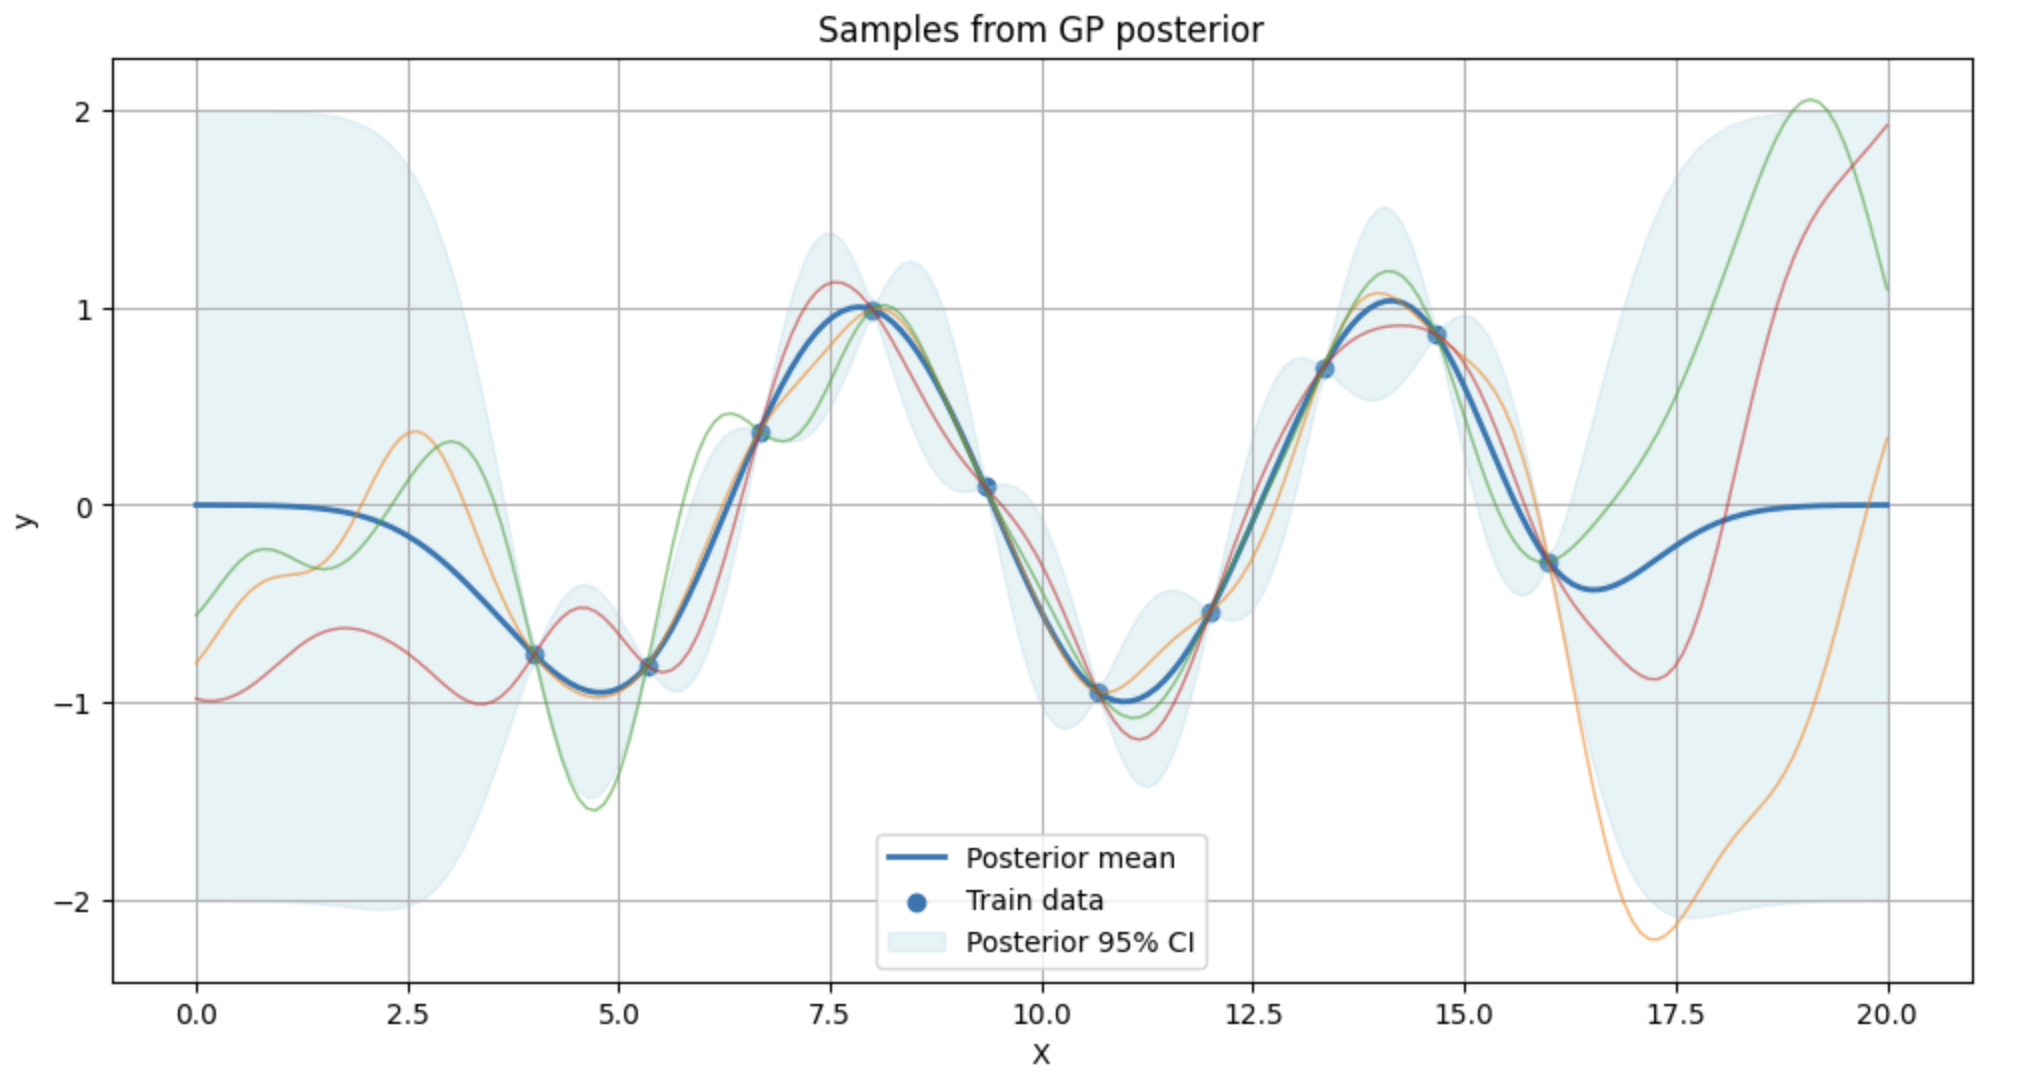
\includegraphics[width=0.8\textwidth]{images/2025-03-08-13-13-53.png}
      \end{center}
    \end{center} 
    Because of our squared exponential kernel, we see that samples are smooth. Instead, if we used $k(x_1 , x_2 ) = \exp (-\norm*{x_1 -x_2 }_{1} )$, our samples would look like:
    \begin{center}
      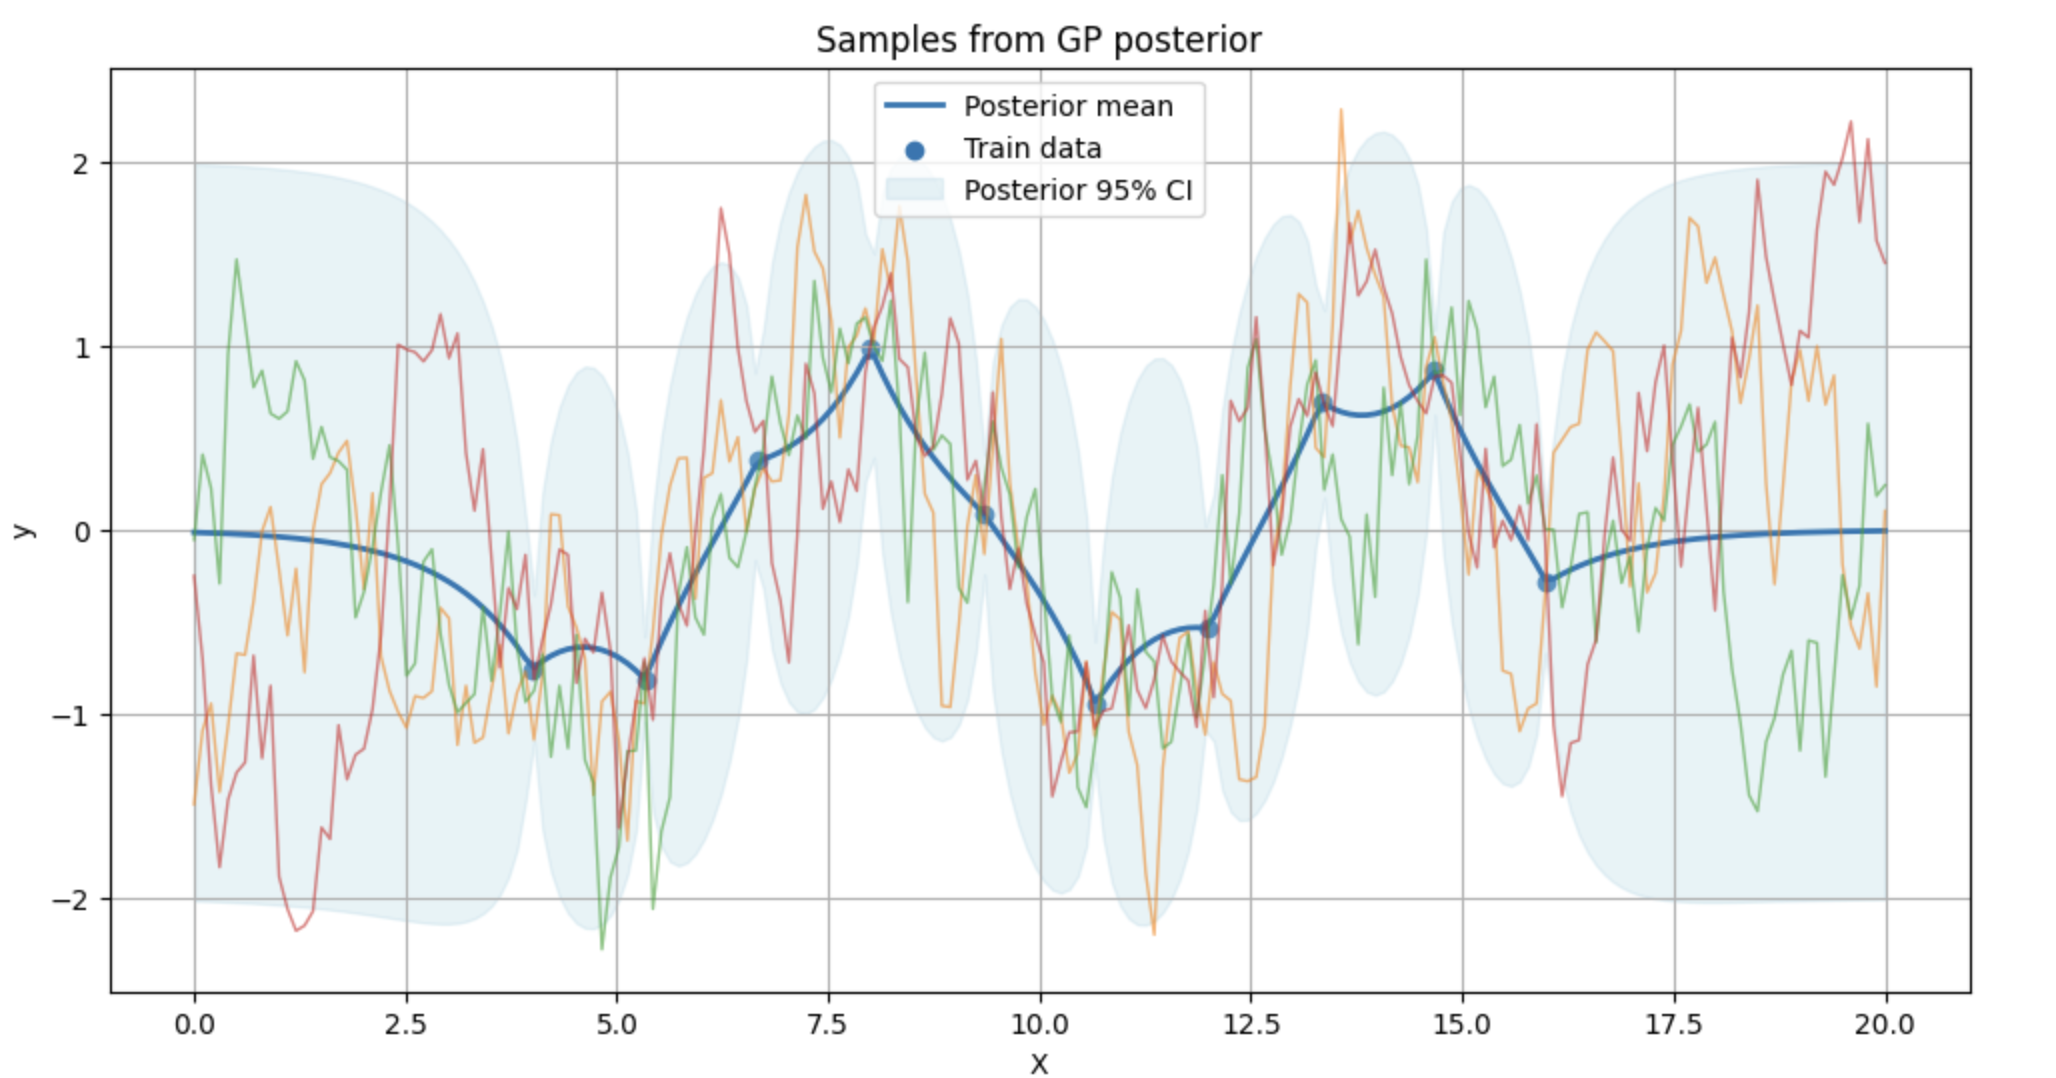
\includegraphics[width=0.8\textwidth]{images/2025-03-08-13-13-10.png}
    \end{center} 
\end{defi}

\section{Posterior of Gaussian process}
A key property of Gaussian processes is that the posterior is also a Gaussian process. The intuition is that we can condition our ``infinite-dimensional'' Gaussian on the outcome $f \coloneqq  f(X)$ of some observed $X$. In particular, by our Gaussian process property, for any test query $X^* $, the joint distribution of $f$ and $f^* \coloneqq f(X^* ) $ is Gaussian:
\[
    N\parens*{\begin{bmatrix}
         \mu (X) \\
         \mu (X^* ) \\
    \end{bmatrix}, 
    \begin{bmatrix}
        K(X, X) &  K(X, X^* ) \\
        K(X^* , X) &  K(X^* , X^* ) \\
    \end{bmatrix}},
\]
Now we can condition on $f$ to get posterior $N(\mu _{f^* \mid D} , \Sigma _{f^* \mid D})$, where 
\begin{align*}
    \mu _{f^* \mid D} &=  \mu (X^* ) + K(X^* , X) K(X, X)^{-1} (f- \mu (X))\\
    \Sigma _{f^* \mid D} &= K(X^* , X^* ) - K(X^* , X) K(X, X)^{-1} K(X, X^* ). 
\end{align*}
In particular, note that these represent valid mean and covariance functions as a function of $X^* $. So the posterior distribution is a Gaussian process. Note that the posterior mean and kernel reflects the visual intuition of our posterior: test points close to data points should have mean close to the observed data values, and near $0$ covariance matrix. 

\section{Noisy observations}
Much like with linear regression, we can assume zero mean noise around our observed datapoints, i.e. 
\[
    y = f + \eps ,
\]
where $\eps \sim N(0, \sigma ^2 )$. Then, the joint distribution of $y, f^* $ becomes
\[
    N\parens*{\begin{bmatrix}
         \mu (X) \\
         \mu (X^* ) \\
    \end{bmatrix}, 
    \begin{bmatrix}
        K(X, X) + \sigma ^2 I &  K(X, X^* ) \\
        K(X^* , X) &  K(X^* , X^* ) \\
    \end{bmatrix}},
\]
As before we condition on $y$ to get posterior on $f^* $ of $N(\mu _{f^* \mid D} , \Sigma _{f^* \mid D})$, where 
\begin{align*}
    \mu _{f^* \mid D} &=  \mu (X^* ) + K(X^* , X) (K(X, X) + \sigma ^2 I)^{-1} (f- \mu (X))\\
    \Sigma _{f^* \mid D} &= K(X^* , X^* ) - K(X^* , X) (K(X, X) + \sigma ^2 I)^{-1} K(X, X^* ). 
\end{align*}

\section{Marginal likelihood}
The marginal likelihood of observed data is an important metric for Bayesian model selection. Assuming again noisy datapoints as well as mean and covariance of our prior parameterized by $\theta $, we have 
\begin{align*}
    p(y \mid x, \theta ) &= \int p(y \mid f) p(f \mid x, \theta ) df\\
    &= \int N(y; f, \sigma ^2 I) N(f; \mu (x;\theta ), K(x, x; \theta )) df\\
    &= N(y; \mu (x; \theta ), \sigma ^2 I + K(x, x;\theta )), 
\end{align*}
by closure of Gaussians under convolution. So the log likelihood is 
\begin{align*}
    &- \frac{1}{2}(y-\mu (x;\theta ))^{\top} (K(x, x;\theta ) 
    + \sigma ^2 I)^{-1} (y-\mu (x; \theta )) \\&- \frac{1}{2}\log \det (K(x, x; \theta ) + \sigma ^2 I) - \frac{N}{2}\log (2\pi ). 
\end{align*}
Note that this incorporates a penalty on the prior covariance (i.e. the complexity of the model). 

\section{Implementation}
\begin{python}
import numpy as np
import matplotlib.pyplot as plt
import math

def f(x):
  return math.sin(x)

def rbf_kernel(x1, x2, length_scale=1.0):
  x1 = x1.reshape(-1, 1)
  x2 = x2.reshape(1, -1)
  return np.exp(-np.square(x1 - x2) / 2 * (length_scale ** 2))

def abs_kernel(x1, x2):
  x1 = x1.reshape(-1, 1)
  x2 = x2.reshape(1, -1)
  return np.exp(-np.abs(x1 - x2))

def gp_posterior(X_train, y_train, X_test, kernel_fn):
  K = kernel_fn(X_train, X_train)  # K(X, X)
  K_s = kernel_fn(X_test, X_train) # K(X^*, X) = K(X, X^*).T
  K_ss = kernel_fn(X_test, X_test) # K(X^*, X^*)

  mu_s = 0 + K_s @ np.linalg.inv(K) @ (y_train - 0)
  cov_s = K_ss - K_s @ np.linalg.inv(K) @ K_s.T
  return mu_s, cov_s
\end{python}

\newpage
\begin{python}
X_train = np.linspace(4, 16, 10)
y_train = np.sin(X_train)
X_test = np.linspace(0, 20, 200)
mu_s, cov_s = gp_posterior(X_train, y_train, X_test, rbf_kernel)
samples = np.random.multivariate_normal(mu_s, cov_s, 3)

plt.figure(figsize=(12, 6))
plt.title('Samples from GP posterior')
plt.xlabel('X')
plt.ylabel('y')
plt.plot(X_test, mu_s, label='Posterior mean', lw=2)
plt.scatter(X_train, y_train, label='Train data')
plt.fill_between(X_test, 
                 mu_s - 2 * np.sqrt(np.diag(cov_s)), 
                 mu_s + 2 * np.sqrt(np.diag(cov_s)), 
                 label='Posterior 95% CI',
                 color='lightblue', alpha=0.3)
for sample in samples:
  plt.plot(X_test, sample, alpha=0.6, lw=1)
plt.grid()
plt.legend()
plt.show()
\end{python}

\end{document}